\chapter{Исследовательский раздел}

В данном разделе приведены технические характеристики устройства, на котором проводилось измерение времени работы программного обеспечения, а также результаты замеров времени работы программы.


\section{Постановка эксперимента}

Целью эксперимента является провести анализ скорости работы алгоритма морфинга изображений с использованием алгоритма Z-буфера для визуализации.

\subsection{Технические характеристики}

Технические характеристики устройства, на котором выполнялось тестирование:
\begin{enumerate}
	\item Процессор Intel(R) Core(TM) i7-11700K @ 3.60GHz;
	\item Оперативная память 32 GB (31.8 GB usable).
\end{enumerate}

Во время тестирования программа была запущена на виртуальной машине Ubuntu 22.04 из операционной системы Windows 11. 
Технические характеристики виртуальной машины:
\begin{enumerate}
	\item Число ядер - 4;
	\item Оперативная память - 20.9 GB.
\end{enumerate}

\subsection{Результаты эксперимента}

Для исследования зависимости времени от размеров фигуры использовались фигуры с различным числом граней и вершин. 
На графиках учитываются грани и вершины результирующих фигур, так как до начала морфинга каждая фигура достраивается либо разрушается так, чтобы количество вершин и граней стало таким же, как у фигуры, к которой она будет преобразована. 
Для каждого случая было проведено по 10 тестов, выбрано среднее значение по времени. 
Результаты эксперимента представлены на рисунке~\ref{fig:res_tests.pdf}.

\begin{figure}[h]
	\centering
	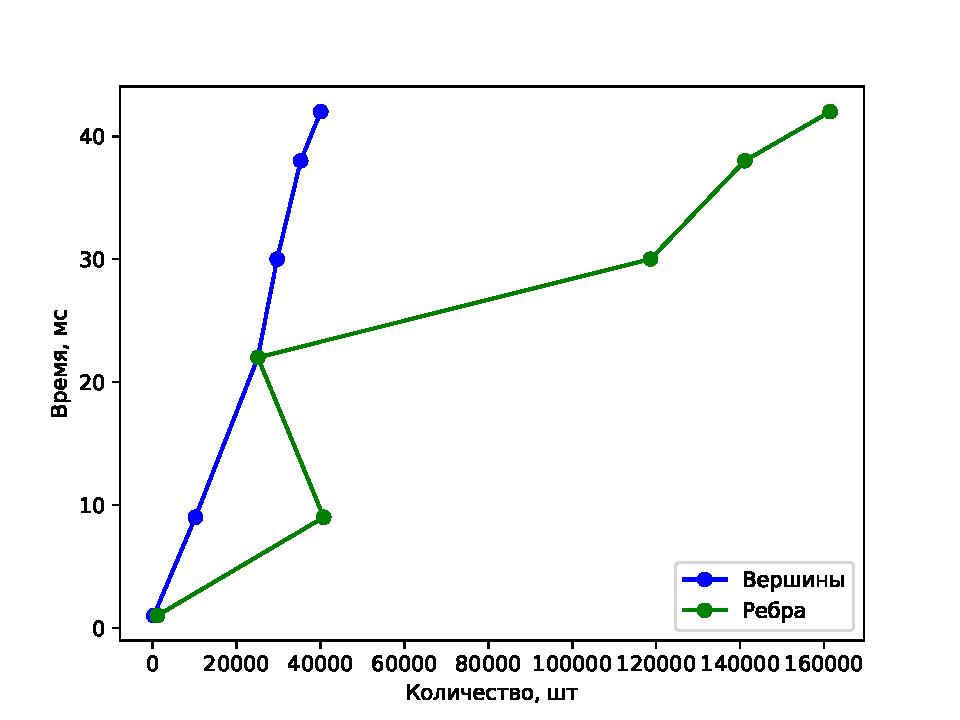
\includegraphics{images/tests.pdf}
	\caption{Результаты эксперимента}
	\label{fig:res_tests.pdf}
\end{figure}

Из проведенного эксперимента можно сделать вывод, что время визуализации сцены во время морфинга линейно зависит от количества вершин результирующей фигуры и слабо зависит от количества граней.

\section*{Выводы из исследовательского раздела}

В данном разделе приведены результаты работы программного обеспечения и проведен эксперимент, показывающий зависимость времени визуализации сцены во время морфинга от количества вершин и ребер результирующей фигуры.

Результаты эксперимента совпали с ожидаемыми, так как в ходе эксперимента было установлено, что время работы увеличивается с увеличением количества вершин и ребер у объекта.
